\chapter{Đường đi ngắn nhất}

\index{đường đi ngắn nhất}

Tìm một đường đi ngắn nhất giữa hai nút
của một đồ thị
là một bài toán quan trọng có nhiều
ứng dụng thực tế.
Ví dụ, một bài toán tự nhiên liên quan đến mạng lưới đường bộ
là tính toán độ dài ngắn nhất có thể của một tuyến đường
giữa hai thành phố, cho biết độ dài của các con đường.

Trong một đồ thị không có trọng số, độ dài của một đường đi bằng
số cạnh của nó, và chúng ta có thể
đơn giản sử dụng tìm kiếm theo chiều rộng để tìm
một đường đi ngắn nhất.
Tuy nhiên, trong chương này chúng ta tập trung vào
các đồ thị có trọng số
nơi cần các thuật toán phức tạp hơn
để tìm đường đi ngắn nhất.

\section{Thuật toán Bellman–Ford}

\index{Thuật toán Bellman–Ford}

\key{Thuật toán Bellman–Ford}\footnote{Thuật toán được đặt theo tên của
R. E. Bellman và L. R. Ford, những người đã công bố nó một cách độc lập
vào năm 1958 và 1956, tương ứng \cite{bel58,for56a}.} tìm
các đường đi ngắn nhất từ một nút bắt đầu đến tất cả
các nút của đồ thị.
Thuật toán có thể xử lý tất cả các loại đồ thị,
miễn là đồ thị không chứa một
chu trình có độ dài âm.
Nếu đồ thị chứa một chu trình âm,
thuật toán có thể phát hiện ra điều này.

Thuật toán theo dõi các khoảng cách
từ nút bắt đầu đến tất cả các nút của đồ thị.
Ban đầu, khoảng cách đến nút bắt đầu là 0
và khoảng cách đến tất cả các nút khác là vô cùng.
Thuật toán giảm các khoảng cách bằng cách tìm
các cạnh rút ngắn các đường đi cho đến khi không
thể giảm bất kỳ khoảng cách nào nữa.

\subsubsection{Ví dụ}

Chúng ta hãy xem xét cách thuật toán Bellman–Ford
hoạt động trong đồ thị sau:
\begin{center}
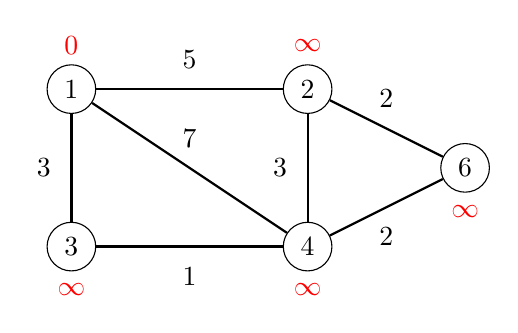
\begin{tikzpicture}
\node[draw, circle] (1) at (1,3) {1};
\node[draw, circle] (2) at (4,3) {2};
\node[draw, circle] (3) at (1,1) {3};
\node[draw, circle] (4) at (4,1) {4};
\node[draw, circle] (5) at (6,2) {6};
\node[color=red] at (1,3+0.55) {$0$};
\node[color=red] at (4,3+0.55) {$\infty$};
\node[color=red] at (1,1-0.55) {$\infty$};
\node[color=red] at (4,1-0.55) {$\infty$};
\node[color=red] at (6,2-0.55) {$\infty$};
\path[draw,thick,-] (1) -- node[font=\small,label=above:5] {} (2);
\path[draw,thick,-] (1) -- node[font=\small,label=left:3] {} (3);
\path[draw,thick,-] (3) -- node[font=\small,label=below:1] {} (4);
\path[draw,thick,-] (2) -- node[font=\small,label=left:3] {} (4);
\path[draw,thick,-] (2) -- node[font=\small,label=above:2] {} (5);
\path[draw,thick,-] (4) -- node[font=\small,label=below:2] {} (5);
\path[draw,thick,-] (1) -- node[font=\small,label=above:7] {} (4);
\end{tikzpicture}
\end{center}
Mỗi nút của đồ thị được gán một khoảng cách.
Ban đầu, khoảng cách đến nút bắt đầu là 0,
và khoảng cách đến tất cả các nút khác là vô cùng.

Thuật toán tìm kiếm các cạnh làm giảm khoảng cách.
Đầu tiên, tất cả các cạnh từ nút 1 làm giảm khoảng cách:
\begin{center}
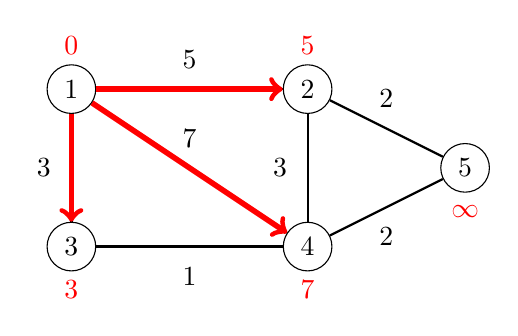
\begin{tikzpicture}
\node[draw, circle] (1) at (1,3) {1};
\node[draw, circle] (2) at (4,3) {2};
\node[draw, circle] (3) at (1,1) {3};
\node[draw, circle] (4) at (4,1) {4};
\node[draw, circle] (5) at (6,2) {5};
\node[color=red] at (1,3+0.55) {$0$};
\node[color=red] at (4,3+0.55) {$5$};
\node[color=red] at (1,1-0.55) {$3$};
\node[color=red] at (4,1-0.55) {$7$};
\node[color=red] at (6,2-0.55) {$\infty$};
\path[draw,thick,-] (1) -- node[font=\small,label=above:5] {} (2);
\path[draw,thick,-] (1) -- node[font=\small,label=left:3] {} (3);
\path[draw,thick,-] (3) -- node[font=\small,label=below:1] {} (4);
\path[draw,thick,-] (2) -- node[font=\small,label=left:3] {} (4);
\path[draw,thick,-] (2) -- node[font=\small,label=above:2] {} (5);
\path[draw,thick,-] (4) -- node[font=\small,label=below:2] {} (5);
\path[draw,thick,-] (1) -- node[font=\small,label=above:7] {} (4);

\path[draw=red,thick,->,line width=2pt] (1) -- (2);
\path[draw=red,thick,->,line width=2pt] (1) -- (3);
\path[draw=red,thick,->,line width=2pt] (1) -- (4);
\end{tikzpicture}
\end{center}
Sau đó, các cạnh
$2 \rightarrow 5$ và $3 \rightarrow 4$
làm giảm khoảng cách:
\begin{center}
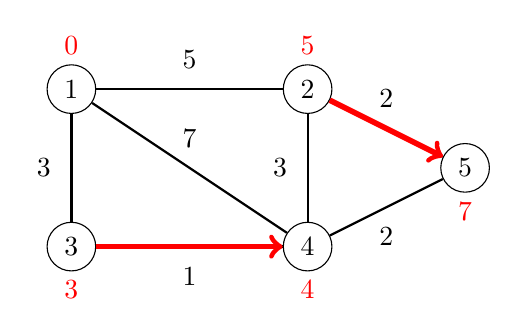
\begin{tikzpicture}
\node[draw, circle] (1) at (1,3) {1};
\node[draw, circle] (2) at (4,3) {2};
\node[draw, circle] (3) at (1,1) {3};
\node[draw, circle] (4) at (4,1) {4};
\node[draw, circle] (5) at (6,2) {5};
\node[color=red] at (1,3+0.55) {$0$};
\node[color=red] at (4,3+0.55) {$5$};
\node[color=red] at (1,1-0.55) {$3$};
\node[color=red] at (4,1-0.55) {$4$};
\node[color=red] at (6,2-0.55) {$7$};
\path[draw,thick,-] (1) -- node[font=\small,label=above:5] {} (2);
\path[draw,thick,-] (1) -- node[font=\small,label=left:3] {} (3);
\path[draw,thick,-] (3) -- node[font=\small,label=below:1] {} (4);
\path[draw,thick,-] (2) -- node[font=\small,label=left:3] {} (4);
\path[draw,thick,-] (2) -- node[font=\small,label=above:2] {} (5);
\path[draw,thick,-] (4) -- node[font=\small,label=below:2] {} (5);
\path[draw,thick,-] (1) -- node[font=\small,label=above:7] {} (4);

\path[draw=red,thick,->,line width=2pt] (2) -- (5);
\path[draw=red,thick,->,line width=2pt] (3) -- (4);
\end{tikzpicture}
\end{center}
Cuối cùng, có một thay đổi nữa:
\begin{center}
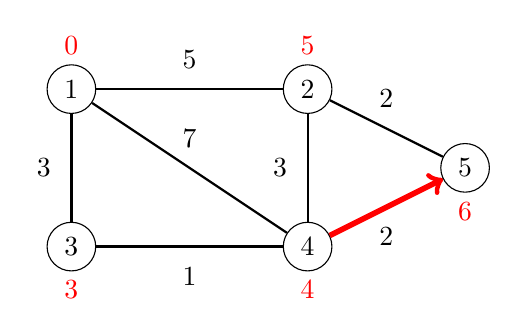
\begin{tikzpicture}
\node[draw, circle] (1) at (1,3) {1};
\node[draw, circle] (2) at (4,3) {2};
\node[draw, circle] (3) at (1,1) {3};
\node[draw, circle] (4) at (4,1) {4};
\node[draw, circle] (5) at (6,2) {5};
\node[color=red] at (1,3+0.55) {$0$};
\node[color=red] at (4,3+0.55) {$5$};
\node[color=red] at (1,1-0.55) {$3$};
\node[color=red] at (4,1-0.55) {$4$};
\node[color=red] at (6,2-0.55) {$6$};
\path[draw,thick,-] (1) -- node[font=\small,label=above:5] {} (2);
\path[draw,thick,-] (1) -- node[font=\small,label=left:3] {} (3);
\path[draw,thick,-] (3) -- node[font=\small,label=below:1] {} (4);
\path[draw,thick,-] (2) -- node[font=\small,label=left:3] {} (4);
\path[draw,thick,-] (2) -- node[font=\small,label=above:2] {} (5);
\path[draw,thick,-] (4) -- node[font=\small,label=below:2] {} (5);
\path[draw,thick,-] (1) -- node[font=\small,label=above:7] {} (4);

\path[draw=red,thick,->,line width=2pt] (4) -- (5);
\end{tikzpicture}
\end{center}

Sau đó, không có cạnh nào có thể làm giảm bất kỳ khoảng cách nào.
Điều này có nghĩa là các khoảng cách là cuối cùng,
và chúng ta đã thành công
tính toán các khoảng cách ngắn nhất
từ nút bắt đầu đến tất cả các nút của đồ thị.

Ví dụ, khoảng cách ngắn nhất 3
từ nút 1 đến nút 5 tương ứng với
đường đi sau:

\begin{center}
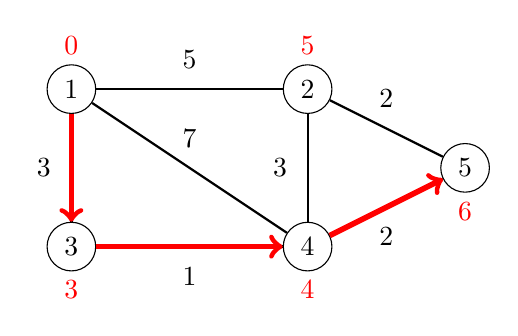
\begin{tikzpicture}
\node[draw, circle] (1) at (1,3) {1};
\node[draw, circle] (2) at (4,3) {2};
\node[draw, circle] (3) at (1,1) {3};
\node[draw, circle] (4) at (4,1) {4};
\node[draw, circle] (5) at (6,2) {5};
\node[color=red] at (1,3+0.55) {$0$};
\node[color=red] at (4,3+0.55) {$5$};
\node[color=red] at (1,1-0.55) {$3$};
\node[color=red] at (4,1-0.55) {$4$};
\node[color=red] at (6,2-0.55) {$6$};
\path[draw,thick,-] (1) -- node[font=\small,label=above:5] {} (2);
\path[draw,thick,-] (1) -- node[font=\small,label=left:3] {} (3);
\path[draw,thick,-] (3) -- node[font=\small,label=below:1] {} (4);
\path[draw,thick,-] (2) -- node[font=\small,label=left:3] {} (4);
\path[draw,thick,-] (2) -- node[font=\small,label=above:2] {} (5);
\path[draw,thick,-] (4) -- node[font=\small,label=below:2] {} (5);
\path[draw,thick,-] (1) -- node[font=\small,label=above:7] {} (4);

\path[draw=red,thick,->,line width=2pt] (1) -- (3);
\path[draw=red,thick,->,line width=2pt] (3) -- (4);
\path[draw=red,thick,->,line width=2pt] (4) -- (5);
\end{tikzpicture}
\end{center}

\subsubsection{Cài đặt}

Cài đặt sau của
thuật toán Bellman–Ford xác định các khoảng cách ngắn nhất
từ một nút $x$ đến tất cả các nút của đồ thị.
Mã giả định rằng đồ thị được lưu trữ
dưới dạng một danh sách cạnh \texttt{edges}
bao gồm các bộ ba có dạng $(a,b,w)$,
nghĩa là có một cạnh từ nút $a$ đến nút $b$
với trọng số $w$.

Thuật toán bao gồm $n-1$ vòng,
và ở mỗi vòng, thuật toán đi qua
tất cả các cạnh của đồ thị và cố gắng
giảm các khoảng cách.
Thuật toán xây dựng một mảng \texttt{distance}
sẽ chứa các khoảng cách từ $x$
đến tất cả các nút của đồ thị.
Hằng số \texttt{INF} biểu thị một khoảng cách vô cùng.

\begin{lstlisting}
for (int i = 1; i <= n; i++) distance[i] = INF;
distance[x] = 0;
for (int i = 1; i <= n-1; i++) {
    for (auto e : edges) {
        int a, b, w;
        tie(a, b, w) = e;
        distance[b] = min(distance[b], distance[a]+w);
    }
}
\end{lstlisting}

Độ phức tạp thời gian của thuật toán là $O(nm)$,
bởi vì thuật toán bao gồm $n-1$ vòng và
lặp qua tất cả $m$ cạnh trong một vòng.
Nếu không có chu trình âm trong đồ thị,
tất cả các khoảng cách là cuối cùng sau $n-1$ vòng,
bởi vì mỗi đường đi ngắn nhất có thể chứa nhiều nhất $n-1$ cạnh.

Trong thực tế, các khoảng cách cuối cùng thường có thể
được tìm thấy nhanh hơn so với $n-1$ vòng.
Do đó, một cách khả thi để làm cho thuật toán hiệu quả hơn
là dừng thuật toán nếu không có khoảng cách nào
có thể được giảm trong một vòng.

\subsubsection{Chu trình âm}

\index{chu trình âm}

Thuật toán Bellman–Ford cũng có thể được sử dụng để
kiểm tra xem đồ thị có chứa một chu trình có độ dài âm hay không.
Ví dụ, đồ thị

\begin{center}
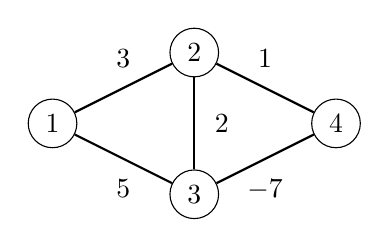
\begin{tikzpicture}[scale=0.9]
\node[draw, circle] (1) at (0,0) {$1$};
\node[draw, circle] (2) at (2,1) {$2$};
\node[draw, circle] (3) at (2,-1) {$3$};
\node[draw, circle] (4) at (4,0) {$4$};

\path[draw,thick,-] (1) -- node[font=\small,label=above:$3$] {} (2);
\path[draw,thick,-] (2) -- node[font=\small,label=above:$1$] {} (4);
\path[draw,thick,-] (1) -- node[font=\small,label=below:$5$] {} (3);
\path[draw,thick,-] (3) -- node[font=\small,label=below:$-7$] {} (4);
\path[draw,thick,-] (2) -- node[font=\small,label=right:$2$] {} (3);
\end{tikzpicture}
\end{center}
\noindent
chứa một chu trình âm
$2 \rightarrow 3 \rightarrow 4 \rightarrow 2$
với độ dài $-4$.

Nếu đồ thị chứa một chu trình âm,
chúng ta có thể rút ngắn vô hạn lần
bất kỳ đường đi nào chứa chu trình bằng cách lặp lại chu trình
liên tục.
Do đó, khái niệm về một đường đi ngắn nhất
không có ý nghĩa trong tình huống này.

Một chu trình âm có thể được phát hiện
bằng cách sử dụng thuật toán Bellman–Ford bằng cách
chạy thuật toán trong $n$ vòng.
Nếu vòng cuối cùng làm giảm bất kỳ khoảng cách nào,
đồ thị chứa một chu trình âm.
Lưu ý rằng thuật toán này có thể được sử dụng để
tìm kiếm
một chu trình âm trong toàn bộ đồ thị
bất kể nút bắt đầu.

\subsubsection{Thuật toán SPFA}

\index{Thuật toán SPFA}

\key{Thuật toán SPFA} (''Shortest Path Faster Algorithm'') \cite{fan94}
là một biến thể của thuật toán Bellman–Ford,
thường hiệu quả hơn thuật toán ban đầu.
Thuật toán SPFA không đi qua tất cả các cạnh trong mỗi vòng,
thay vào đó, nó chọn các cạnh để kiểm tra
một cách thông minh hơn.

Thuật toán duy trì một hàng đợi các nút có thể
được sử dụng để giảm khoảng cách.
Đầu tiên, thuật toán thêm nút bắt đầu $x$
vào hàng đợi.
Sau đó, thuật toán luôn xử lý
nút đầu tiên trong hàng đợi, và khi một cạnh
$a \rightarrow b$ làm giảm khoảng cách,
nút $b$ được thêm vào hàng đợi.
% 
% The following implementation uses a 
% \texttt{queue} \texttt{q}.
% In addition, an array \texttt{inqueue} indicates
% if a node is already in the queue,
% in which case the algorithm does not add
% the node to the queue again.
% 
% \begin{lstlisting}
% for (int i = 1; i <= n; i++) distance[i] = INF;
% distance[x] = 0;
% q.push(x);
% while (!q.empty()) {
%     int a = q.front(); q.pop();
%     inqueue[a] = false;
%     for (auto b : v[a]) {
%         if (distance[a]+b.second < distance[b.first]) {
%             distance[b.first] = distance[a]+b.second;
%             if (!inqueue[b]) {q.push(b); inqueue[b] = true;}
%         }
%     }
% }
% \end{lstlisting}

Hiệu quả của thuật toán SPFA phụ thuộc
vào cấu trúc của đồ thị:
thuật toán thường hiệu quả,
nhưng độ phức tạp thời gian trường hợp xấu nhất của nó vẫn là
$O(nm)$ và có thể tạo ra các đầu vào
làm cho thuật toán chậm như
thuật toán Bellman–Ford ban đầu.

\section{Thuật toán Dijkstra}

\index{Thuật toán Dijkstra}

\key{Thuật toán Dijkstra}\footnote{E. W. Dijkstra đã công bố thuật toán vào năm 1959 \cite{dij59};
tuy nhiên, bài báo gốc của ông không đề cập đến cách cài đặt thuật toán một cách hiệu quả.}
tìm các đường đi ngắn nhất từ nút bắt đầu đến tất cả các nút của đồ thị,
giống như thuật toán Bellman–Ford.
Lợi ích của thuật toán Dijsktra là
nó hiệu quả hơn và có thể được sử dụng để
xử lý các đồ thị lớn.
Tuy nhiên, thuật toán yêu cầu không có
cạnh trọng số âm trong đồ thị.

Giống như thuật toán Bellman–Ford,
thuật toán Dijkstra duy trì khoảng cách
đến các nút và giảm chúng trong quá trình tìm kiếm.
Thuật toán Dijkstra hiệu quả, bởi vì
nó chỉ xử lý
mỗi cạnh trong đồ thị một lần, sử dụng thực tế
rằng không có cạnh âm.

\subsubsection{Ví dụ}

Chúng ta hãy xem xét cách thuật toán Dijkstra
hoạt động trong đồ thị sau khi
nút bắt đầu là nút 1:
\begin{center}
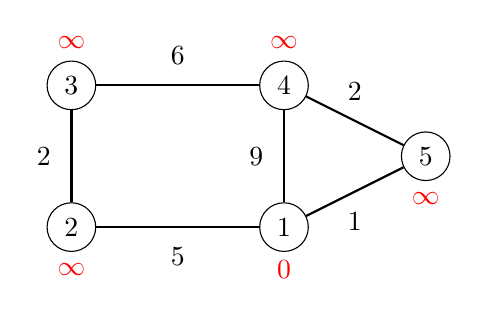
\begin{tikzpicture}[scale=0.9]
\node[draw, circle] (1) at (1,3) {3};
\node[draw, circle] (2) at (4,3) {4};
\node[draw, circle] (3) at (1,1) {2};
\node[draw, circle] (4) at (4,1) {1};
\node[draw, circle] (5) at (6,2) {5};

\node[color=red] at (1,3+0.6) {$\infty$};
\node[color=red] at (4,3+0.6) {$\infty$};
\node[color=red] at (1,1-0.6) {$\infty$};
\node[color=red] at (4,1-0.6) {$0$};
\node[color=red] at (6,2-0.6) {$\infty$};

\path[draw,thick,-] (1) -- node[font=\small,label=above:6] {} (2);
\path[draw,thick,-] (1) -- node[font=\small,label=left:2] {} (3);
\path[draw,thick,-] (3) -- node[font=\small,label=below:5] {} (4);
\path[draw,thick,-] (2) -- node[font=\small,label=left:9] {} (4);
\path[draw,thick,-] (2) -- node[font=\small,label=above:2] {} (5);
\path[draw,thick,-] (4) -- node[font=\small,label=below:1] {} (5);
\end{tikzpicture}
\end{center}
Giống như trong thuật toán Bellman–Ford,
ban đầu khoảng cách đến nút bắt đầu là 0
và khoảng cách đến tất cả các nút khác là vô cùng.

Tại mỗi bước, thuật toán Dijkstra chọn một nút
chưa được xử lý và có khoảng cách
nhỏ nhất có thể.
Nút đầu tiên như vậy là nút 1 với khoảng cách 0.

Khi một nút được chọn, thuật toán
đi qua tất cả các cạnh bắt đầu tại nút đó
và giảm khoảng cách bằng cách sử dụng chúng:
\begin{center}
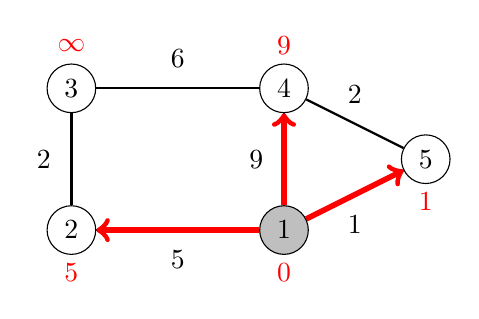
\begin{tikzpicture}[scale=0.9]
\node[draw, circle] (1) at (1,3) {3};
\node[draw, circle] (2) at (4,3) {4};
\node[draw, circle] (3) at (1,1) {2};
\node[draw, circle, fill=lightgray] (4) at (4,1) {1};
\node[draw, circle] (5) at (6,2) {5};

\node[color=red] at (1,3+0.6) {$\infty$};
\node[color=red] at (4,3+0.6) {$9$};
\node[color=red] at (1,1-0.6) {$5$};
\node[color=red] at (4,1-0.6) {$0$};
\node[color=red] at (6,2-0.6) {$1$};

\path[draw,thick,-] (1) -- node[font=\small,label=above:6] {} (2);
\path[draw,thick,-] (1) -- node[font=\small,label=left:2] {} (3);
\path[draw,thick,-] (3) -- node[font=\small,label=below:5] {} (4);
\path[draw,thick,-] (2) -- node[font=\small,label=left:9] {} (4);
\path[draw,thick,-] (2) -- node[font=\small,label=above:2] {} (5);
\path[draw,thick,-] (4) -- node[font=\small,label=below:1] {} (5);

\path[draw=red,thick,->,line width=2pt] (4) -- (2);
\path[draw=red,thick,->,line width=2pt] (4) -- (3);
\path[draw=red,thick,->,line width=2pt] (4) -- (5);
\end{tikzpicture}
\end{center}
Trong trường hợp này,
các cạnh từ nút 1 đã giảm khoảng cách của
các nút 2, 4 và 5, có khoảng cách bây giờ là 5, 9 và 1.

Nút tiếp theo được xử lý là nút 5 với khoảng cách 1.
Điều này làm giảm khoảng cách đến nút 4 từ 9 xuống 3:
\begin{center}
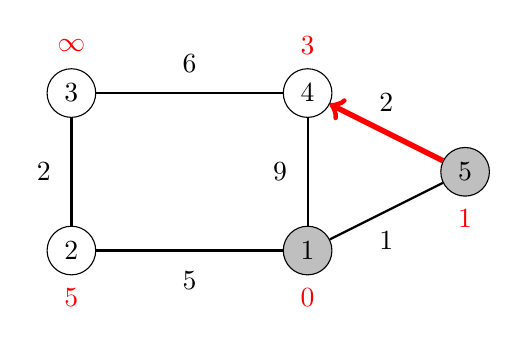
\begin{tikzpicture}
\node[draw, circle] (1) at (1,3) {3};
\node[draw, circle] (2) at (4,3) {4};
\node[draw, circle] (3) at (1,1) {2};
\node[draw, circle, fill=lightgray] (4) at (4,1) {1};
\node[draw, circle, fill=lightgray] (5) at (6,2) {5};

\node[color=red] at (1,3+0.6) {$\infty$};
\node[color=red] at (4,3+0.6) {$3$};
\node[color=red] at (1,1-0.6) {$5$};
\node[color=red] at (4,1-0.6) {$0$};
\node[color=red] at (6,2-0.6) {$1$};

\path[draw,thick,-] (1) -- node[font=\small,label=above:6] {} (2);
\path[draw,thick,-] (1) -- node[font=\small,label=left:2] {} (3);
\path[draw,thick,-] (3) -- node[font=\small,label=below:5] {} (4);
\path[draw,thick,-] (2) -- node[font=\small,label=left:9] {} (4);
\path[draw,thick,-] (2) -- node[font=\small,label=above:2] {} (5);
\path[draw,thick,-] (4) -- node[font=\small,label=below:1] {} (5);

\path[draw=red,thick,->,line width=2pt] (5) -- (2);
\end{tikzpicture}
\end{center}
Sau đó, nút tiếp theo là nút 4, làm giảm
khoảng cách đến nút 3 xuống 9:
\begin{center}
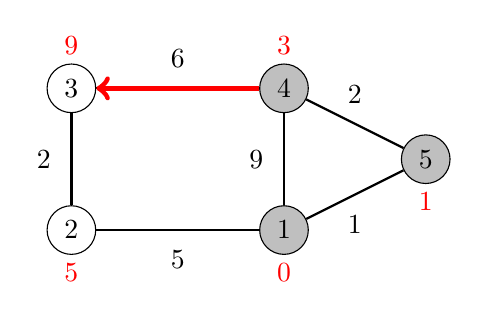
\begin{tikzpicture}[scale=0.9]
\node[draw, circle] (1) at (1,3) {3};
\node[draw, circle, fill=lightgray] (2) at (4,3) {4};
\node[draw, circle] (3) at (1,1) {2};
\node[draw, circle, fill=lightgray] (4) at (4,1) {1};
\node[draw, circle, fill=lightgray] (5) at (6,2) {5};

\node[color=red] at (1,3+0.6) {$9$};
\node[color=red] at (4,3+0.6) {$3$};
\node[color=red] at (1,1-0.6) {$5$};
\node[color=red] at (4,1-0.6) {$0$};
\node[color=red] at (6,2-0.6) {$1$};

\path[draw,thick,-] (1) -- node[font=\small,label=above:6] {} (2);
\path[draw,thick,-] (1) -- node[font=\small,label=left:2] {} (3);
\path[draw,thick,-] (3) -- node[font=\small,label=below:5] {} (4);
\path[draw,thick,-] (2) -- node[font=\small,label=left:9] {} (4);
\path[draw,thick,-] (2) -- node[font=\small,label=above:2] {} (5);
\path[draw,thick,-] (4) -- node[font=\small,label=below:1] {} (5);

\path[draw=red,thick,->,line width=2pt] (2) -- (1);
\end{tikzpicture}
\end{center}

Một thuộc tính đáng chú ý trong thuật toán Dijkstra là
bất cứ khi nào một nút được chọn, khoảng cách của nó là cuối cùng.
Ví dụ, tại thời điểm này của thuật toán,
các khoảng cách 0, 1 và 3 là các khoảng cách cuối cùng
đến các nút 1, 5 và 4.

Sau đó, thuật toán xử lý hai
nút còn lại, và các khoảng cách cuối cùng như sau:

\begin{center}
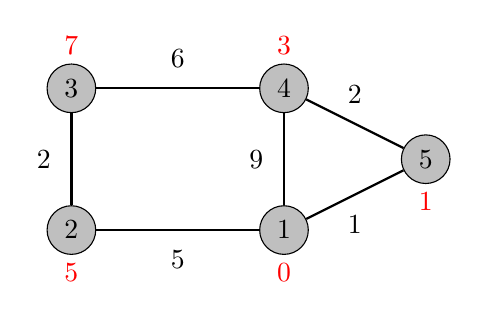
\begin{tikzpicture}[scale=0.9]
\node[draw, circle, fill=lightgray] (1) at (1,3) {3};
\node[draw, circle, fill=lightgray] (2) at (4,3) {4};
\node[draw, circle, fill=lightgray] (3) at (1,1) {2};
\node[draw, circle, fill=lightgray] (4) at (4,1) {1};
\node[draw, circle, fill=lightgray] (5) at (6,2) {5};

\node[color=red] at (1,3+0.6) {$7$};
\node[color=red] at (4,3+0.6) {$3$};
\node[color=red] at (1,1-0.6) {$5$};
\node[color=red] at (4,1-0.6) {$0$};
\node[color=red] at (6,2-0.6) {$1$};

\path[draw,thick,-] (1) -- node[font=\small,label=above:6] {} (2);
\path[draw,thick,-] (1) -- node[font=\small,label=left:2] {} (3);
\path[draw,thick,-] (3) -- node[font=\small,label=below:5] {} (4);
\path[draw,thick,-] (2) -- node[font=\small,label=left:9] {} (4);
\path[draw,thick,-] (2) -- node[font=\small,label=above:2] {} (5);
\path[draw,thick,-] (4) -- node[font=\small,label=below:1] {} (5);
\end{tikzpicture}
\end{center}

\subsubsection{Cạnh âm}

Hiệu quả của thuật toán Dijkstra
dựa trên thực tế là đồ thị không
chứa các cạnh âm.
Nếu có một cạnh âm,
thuật toán có thể cho kết quả không chính xác.
Ví dụ, hãy xem xét đồ thị sau:

\begin{center}
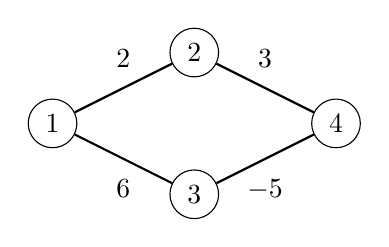
\begin{tikzpicture}[scale=0.9]
\node[draw, circle] (1) at (0,0) {$1$};
\node[draw, circle] (2) at (2,1) {$2$};
\node[draw, circle] (3) at (2,-1) {$3$};
\node[draw, circle] (4) at (4,0) {$4$};

\path[draw,thick,-] (1) -- node[font=\small,label=above:2] {} (2);
\path[draw,thick,-] (2) -- node[font=\small,label=above:3] {} (4);
\path[draw,thick,-] (1) -- node[font=\small,label=below:6] {} (3);
\path[draw,thick,-] (3) -- node[font=\small,label=below:$-5$] {} (4);
\end{tikzpicture}
\end{center}
\noindent
Đường đi ngắn nhất từ nút 1 đến nút 4 là
$1 \rightarrow 3 \rightarrow 4$
và độ dài của nó là 1.
Tuy nhiên, thuật toán Dijkstra
tìm thấy đường đi $1 \rightarrow 2 \rightarrow 4$
bằng cách đi theo các cạnh có trọng số nhỏ nhất.
Thuật toán không tính đến việc
trên đường đi kia, trọng số $-5$
bù lại cho trọng số lớn trước đó là $6$.

\subsubsection{Cài đặt}

Cài đặt sau của thuật toán Dijkstra
tính toán khoảng cách nhỏ nhất từ một nút $x$
đến các nút khác của đồ thị.
Đồ thị được lưu trữ dưới dạng danh sách kề
sao cho \texttt{adj[$a$]} chứa một cặp $(b,w)$
luôn luôn khi có một cạnh từ nút $a$ đến nút $b$
với trọng số $w$.

Một cài đặt hiệu quả của thuật toán Dijkstra
yêu cầu có thể tìm thấy hiệu quả
nút có khoảng cách nhỏ nhất chưa được xử lý.
Một cấu trúc dữ liệu thích hợp cho việc này là hàng đợi ưu tiên
chứa các nút được sắp xếp theo khoảng cách của chúng.
Sử dụng hàng đợi ưu tiên, nút tiếp theo cần xử lý
có thể được lấy ra trong thời gian logarit.

Trong đoạn mã sau, hàng đợi ưu tiên
\texttt{q} chứa các cặp có dạng $(-d,x)$,
nghĩa là khoảng cách hiện tại đến nút $x$ là $d$.
Mảng $\texttt{distance}$ chứa khoảng cách đến
mỗi nút, và mảng $\texttt{processed}$ chỉ ra
liệu một nút đã được xử lý hay chưa.
Ban đầu khoảng cách là $0$ đến $x$ và $\infty$ đến tất cả các nút khác.

\begin{lstlisting}
for (int i = 1; i <= n; i++) distance[i] = INF;
distance[x] = 0;
q.push({0,x});
while (!q.empty()) {
    int a = q.top().second; q.pop();
    if (processed[a]) continue;
    processed[a] = true;
    for (auto u : adj[a]) {
        int b = u.first, w = u.second;
        if (distance[a]+w < distance[b]) {
            distance[b] = distance[a]+w;
            q.push({-distance[b],b});
        }
    }
}
\end{lstlisting}

Lưu ý rằng hàng đợi ưu tiên chứa các khoảng cách \emph{âm}
đến các nút.
Lý do cho điều này là phiên bản
mặc định của hàng đợi ưu tiên C++ tìm các phần tử
lớn nhất, trong khi chúng ta muốn tìm các phần tử nhỏ nhất.
Bằng cách sử dụng các khoảng cách âm,
chúng ta có thể sử dụng trực tiếp hàng đợi ưu tiên mặc định\footnote{Tất nhiên,
chúng ta cũng có thể khai báo hàng đợi ưu tiên như trong Chương 4.5
và sử dụng các khoảng cách dương, nhưng việc cài đặt sẽ dài hơn một chút.}.
Cũng lưu ý rằng có thể có nhiều phiên bản của cùng một
nút trong hàng đợi ưu tiên; tuy nhiên, chỉ có phiên bản có
khoảng cách nhỏ nhất sẽ được xử lý.

Độ phức tạp thời gian của cài đặt trên là
$O(n+m \log m)$, bởi vì thuật toán đi qua
tất cả các nút của đồ thị và thêm cho mỗi cạnh
nhiều nhất một khoảng cách vào hàng đợi ưu tiên.

\section{Thuật toán Floyd–Warshall}

\index{Thuật toán Floyd–Warshall}

\key{Thuật toán Floyd–Warshall}\footnote{Thuật toán
được đặt theo tên của R. W. Floyd và S. Warshall
những người đã công bố nó một cách độc lập vào năm 1962 \cite{flo62,war62}.}
cung cấp một cách tiếp cận thay thế cho bài toán
tìm đường đi ngắn nhất.
Không giống như các thuật toán khác trong chương này,
nó tìm tất cả các đường đi ngắn nhất giữa các nút
trong một lần chạy duy nhất.

Thuật toán duy trì một mảng hai chiều
chứa khoảng cách giữa các nút.
Đầu tiên, khoảng cách chỉ được tính toán bằng cách sử dụng
các cạnh trực tiếp giữa các nút,
và sau đó, thuật toán giảm khoảng cách
bằng cách sử dụng các nút trung gian trong các đường đi.

\subsubsection{Ví dụ}

Chúng ta hãy xem xét cách thuật toán Floyd–Warshall
hoạt động trong đồ thị sau:

\begin{center}
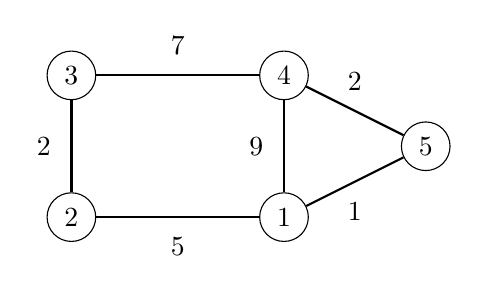
\begin{tikzpicture}[scale=0.9]
\node[draw, circle] (1) at (1,3) {$3$};
\node[draw, circle] (2) at (4,3) {$4$};
\node[draw, circle] (3) at (1,1) {$2$};
\node[draw, circle] (4) at (4,1) {$1$};
\node[draw, circle] (5) at (6,2) {$5$};

\path[draw,thick,-] (1) -- node[font=\small,label=above:7] {} (2);
\path[draw,thick,-] (1) -- node[font=\small,label=left:2] {} (3);
\path[draw,thick,-] (3) -- node[font=\small,label=below:5] {} (4);
\path[draw,thick,-] (2) -- node[font=\small,label=left:9] {} (4);
\path[draw,thick,-] (2) -- node[font=\small,label=above:2] {} (5);
\path[draw,thick,-] (4) -- node[font=\small,label=below:1] {} (5);
\end{tikzpicture}
\end{center}

Ban đầu, khoảng cách từ mỗi nút đến chính nó là $0$,
và khoảng cách giữa các nút $a$ và $b$ là $x$
nếu có một cạnh giữa các nút $a$ và $b$ với trọng số $x$.
Tất cả các khoảng cách khác là vô cùng.

Trong đồ thị này, mảng ban đầu như sau:
\begin{center}
\begin{tabular}{r|rrrrr}
 & 1 & 2 & 3 & 4 & 5 \\
\hline
1 & 0 & 5 & $\infty$ & 9 & 1 \\
2 & 5 & 0 & 2 & $\infty$ & $\infty$ \\
3 & $\infty$ & 2 & 0 & 7 & $\infty$ \\
4 & 9 & $\infty$ & 7 & 0 & 2 \\
5 & 1 & $\infty$ & $\infty$ & 2 & 0 \\
\end{tabular}
\end{center}
\vspace{10pt}
Thuật toán bao gồm các vòng liên tiếp.
Trên mỗi vòng, thuật toán chọn một nút mới
có thể hoạt động như một nút trung gian trong các đường đi từ bây giờ,
và khoảng cách được giảm bằng cách sử dụng nút này.

Ở vòng đầu tiên, nút 1 là nút trung gian mới.
Có một đường đi mới giữa các nút 2 và 4
với độ dài 14, vì nút 1 kết nối chúng.
Cũng có một đường đi mới
giữa các nút 2 và 5 với độ dài 6.

\begin{center}
\begin{tabular}{r|rrrrr}
 & 1 & 2 & 3 & 4 & 5 \\
\hline
1 & 0 & 5 & $\infty$ & 9 & 1 \\
2 & 5 & 0 & 2 & \textbf{14} & \textbf{6} \\
3 & $\infty$ & 2 & 0 & 7 & $\infty$ \\
4 & 9 & \textbf{14} & 7 & 0 & 2 \\
5 & 1 & \textbf{6} & $\infty$ & 2 & 0 \\
\end{tabular}
\end{center}
\vspace{10pt}

Ở vòng thứ hai, nút 2 là nút trung gian mới.
Điều này tạo ra các đường đi mới giữa các nút 1 và 3
và giữa các nút 3 và 5:

\begin{center}
\begin{tabular}{r|rrrrr}
 & 1 & 2 & 3 & 4 & 5 \\
\hline
1 & 0 & 5 & \textbf{7} & 9 & 1 \\
2 & 5 & 0 & 2 & 14 & 6 \\
3 & \textbf{7} & 2 & 0 & 7 & \textbf{8} \\
4 & 9 & 14 & 7 & 0 & 2 \\
5 & 1 & 6 & \textbf{8} & 2 & 0 \\
\end{tabular}
\end{center}
\vspace{10pt}

Ở vòng thứ ba, nút 3 là vòng trung gian mới.
Có một đường đi mới giữa các nút 2 và 4:

\begin{center}
\begin{tabular}{r|rrrrr}
 & 1 & 2 & 3 & 4 & 5 \\
\hline
1 & 0 & 5 & 7 & 9 & 1 \\
2 & 5 & 0 & 2 & \textbf{9} & 6 \\
3 & 7 & 2 & 0 & 7 & 8 \\
4 & 9 & \textbf{9} & 7 & 0 & 2 \\
5 & 1 & 6 & 8 & 2 & 0 \\
\end{tabular}
\end{center}
\vspace{10pt}

Thuật toán tiếp tục như vậy,
cho đến khi tất cả các nút đã được chỉ định làm nút trung gian.
Sau khi thuật toán kết thúc, mảng chứa
khoảng cách tối thiểu giữa bất kỳ hai nút nào:

\begin{center}
\begin{tabular}{r|rrrrr}
 & 1 & 2 & 3 & 4 & 5 \\
\hline
1 & 0 & 5 & 7 & 3 & 1 \\
2 & 5 & 0 & 2 & 8 & 6 \\
3 & 7 & 2 & 0 & 7 & 8 \\
4 & 3 & 8 & 7 & 0 & 2 \\
5 & 1 & 6 & 8 & 2 & 0 \\
\end{tabular}
\end{center}

Ví dụ, mảng cho chúng ta biết rằng
khoảng cách ngắn nhất giữa các nút 2 và 4 là 8.
Điều này tương ứng với đường đi sau:

\begin{center}
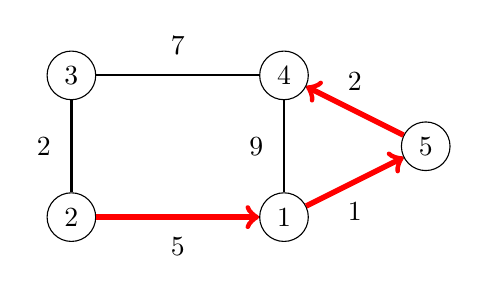
\begin{tikzpicture}[scale=0.9]
\node[draw, circle] (1) at (1,3) {$3$};
\node[draw, circle] (2) at (4,3) {$4$};
\node[draw, circle] (3) at (1,1) {$2$};
\node[draw, circle] (4) at (4,1) {$1$};
\node[draw, circle] (5) at (6,2) {$5$};

\path[draw,thick,-] (1) -- node[font=\small,label=above:7] {} (2);
\path[draw,thick,-] (1) -- node[font=\small,label=left:2] {} (3);
\path[draw,thick,-] (3) -- node[font=\small,label=below:5] {} (4);
\path[draw,thick,-] (2) -- node[font=\small,label=left:9] {} (4);
\path[draw,thick,-] (2) -- node[font=\small,label=above:2] {} (5);
\path[draw,thick,-] (4) -- node[font=\small,label=below:1] {} (5);

\path[draw=red,thick,->,line width=2pt] (3) -- (4);
\path[draw=red,thick,->,line width=2pt] (4) -- (5);
\path[draw=red,thick,->,line width=2pt] (5) -- (2);
\end{tikzpicture}
\end{center}

\subsubsection{Cài đặt}

Ưu điểm của thuật toán
Floyd–Warshall là nó
dễ cài đặt.
Đoạn mã sau xây dựng một
ma trận khoảng cách trong đó $\texttt{distance}[a][b]$
là khoảng cách ngắn nhất giữa các nút $a$ và $b$.
Đầu tiên, thuật toán khởi tạo \texttt{distance}
sử dụng ma trận kề \texttt{adj} của đồ thị:

\begin{lstlisting}
for (int i = 1; i <= n; i++) {
    for (int j = 1; j <= n; j++) {
        if (i == j) distance[i][j] = 0;
        else if (adj[i][j]) distance[i][j] = adj[i][j];
        else distance[i][j] = INF;
    }
}
\end{lstlisting}
Sau đó, các khoảng cách ngắn nhất có thể được tìm thấy như sau:
\begin{lstlisting}
for (int k = 1; k <= n; k++) {
    for (int i = 1; i <= n; i++) {
        for (int j = 1; j <= n; j++) {
            distance[i][j] = min(distance[i][j],
                                   distance[i][k]+distance[k][j]);
        }
    }
}
\end{lstlisting}

Độ phức tạp thời gian của thuật toán là $O(n^3)$,
vì nó chứa ba vòng lặp lồng nhau
đi qua các nút của đồ thị.

Vì việc cài đặt thuật toán Floyd–Warshall
đơn giản, thuật toán có thể là
một lựa chọn tốt ngay cả khi chỉ cần tìm một
đường đi ngắn nhất duy nhất trong đồ thị.
Tuy nhiên, thuật toán chỉ có thể được sử dụng khi đồ thị
đủ nhỏ để độ phức tạp thời gian bậc ba đủ nhanh.
